\documentclass[draftfoot,preprint]{cit_thesis}
\usepackage{graphicx}

\begin{document}

\title{Search for Dark Matter Direct Production in proton-proton collisions at sqrt(s) = 8 TeV With the CMS Detector at the LHC}
\author{Cristian Pe\~na}

\maketitle

\begin{abstract}
A search for dark matter (DM) is carried out....
\end{abstract}

\chapter{Introduction}
% Perharps the best way to introduce the current state of particle
% physics is to start with a historical\footnote{by no means I
%   pretend to have a rigorous historical approach but rather summarize
%   the scientific triumphs that shaped what particle physics is today}
% approach. The beginning of modern particle physics starts in 1897 with the
% discovery of electron by J. J. Thomson while he was studying cathode
% rays. Thompson determined that the charge-to-mass ratio was extremely
% large and therefore a new particle with negative charge and extremely
% light was necessary to explain the observations. Later came, continuing the
% path of what is sometimes called classical particle physics,
% Rutherford's famous scaterring experiment, which by recording the
% angles of the outgoing $\alpha-$particles scaterred off a gold foil,
% reached the astonishing conclusion that the majority of the charge and
% mass of the atom is contained in a small region in space, the
% nucleus. The nucleus of the lightest element -- hydrogen, which has an
% electron orbiting the nucleus -- is what we know as the
% proton. Spectacular agreement between the theoretical predictions and
% the experimental measurements of the spectrum of hydrogen gave
% credibility to atomic model. Thus, it is was proposed that the rest of
% the elements, which are hevier, will have just more protons in the
% nucleus and the corresponding number of electron orbiting it. This
% picture was inmediately proved wrong since the mass of the next
% element, helium, was measure to approximately weigh 4 times as much as
% hydrogen. Although wrong, this model correctly predicted the number of
% electrons. Therefore the somewhat obvious solution was to set the number of protons to match that of electron -- so that the
% net charge of the atom is zero -- and introduce a neutral particle
% with the same mass as the proton, the neutron. The neutron was
% discovered by Chadwick in 1932 and thus completed the atomic
% model. During the same period of time, i.e. 1900-1924, another
% scientific revolution was developing, this revolution will paved the
% road to the priciples of quantum mechanics and proposed a new
% fundamentally different particle, the photon. The photon discovery
% started in 1900, when Planck introduced it in order to explain the
% observed blackbody spectrum -- the spectrum of the
% electromagnetic radiation emitted by a hot object. In order to
% overcome the difficulties of statistical mechanics in explaining the
% blackbody spectrum, Planck had to introduce the radical notion that electromagnetic radiation was \textit{quantized}, this is to say, that
% it only comes in small energy ``packages'' (quanta), these quanta
% carry an energy proportional to the frecuency of the electromagnetic
% radiation ($E = h\nu$). Although this quantization of the energy did
% solve the blackbody spectrum problem, Planck did not believe that the
% quantization was part of reality. By 1905, perhaps the most well know
% physicist, Albert Einsteined proposed that the quantization was indeed
% inherent to the electromagnetic field. He used this idea to explain
% the \textit{photoelectric effect}. When the surface of a metal is hit
% by electromagnetic radiation, electrons are release with a particular
% energy. Einstein argued that a quantum of light transfered all its
% energy ($h\nu$) to an electron, then the excited electron upon
% traveling out of the material will loose a determined amoung of energy
% (the work function, $w$); therefore the energy of the outgoing electron is
% $E\leq h\nu - w$. Despite of the experimental success of the
% photoelectric effect theory, measured by Millikan in 1916, the
% community was not willing to accept the quantization idea as a
% fundamental part of nature. Finally, in 1923 A. Compton
Particle physics is perhaps facing one of the biggest crossroads since
the discovery of the electron in 1987. The subject evolved from having
just one particle to have a catalog of particles and their possible
interactions, and even explain the origen of the particles
masses. This knowledge is encoded in what we today know as the
Standard Model (SM) of particle physics, the most precise and perhaps
the most succesful theory that mankind has ever had. The SM is a
quantum filed theory that sets the
rules by which the particles that we have observed interact with each
other, these interaction comprise three of the four fundamental force
we know: the strong, weak, and electromagnetic interactions; leaving
gravity asside. Most of the predictions since its formulation, mostly
during the 1960s, have been experimentally observed: we have measured the W and Z
bosons, the top quark, and recent the discovery of the last piece of
the puzzle by the ATLAS and CMS collaborations~\cite{CMSHIGGS,ATLASHIGGS}, the Higgs boson. Despite the success and completeness of
the SM, both experimentally and theoretically motivated, we are now
faced with fundamental questions that are unfortunately not answered:

\begin{itemize}
\item What is the nature of the \textit{dark matter} whose existance
  has only been inferred by astrophysical measurement?
\item Is there a unification of the gauge coupling at the Planck scale?
\item Why is Higgs boson mass at the weak scale since its mass is
  sensitive to a high energy scale through radiative corrections (fine
  tunning)?
\item What's the nature of the matter/anti-matter assymetry observed
  in the universe?
\item  What is the nature of \textit{dark energy} whose existence provides an
  explanation for the expansion of the universe?
\item Is there a quantum theory of gravity?
\end{itemize} 

This thesis is more concerned with the first three bullets, which can
actually be answerd with a single theory: \textit{supersymmetry}, a
quantum field theory that relates fermions and bosons\cite{xx}, which tackles
these questions by adding a dark matter candidate to the
particle spectrum, unifiying the gauge couplings at the Planck scale,
and alleviating the fine tunning of the Higgs mass.

Although suppersymetry is a very compeling theoretical framework, it is not needed for having
a suitable dark matter candidate. In fact, in order to match
the observed dark matter relic density, there are just two
conditions that need to be satisfied. These are, the strength of the interaction of the dark matter (DM)
candidate -- here it is assumed that the DM candidate is a fundamental
particle -- with the SM particles is at the level of the weak interaction,
and the mass of the DM candidate is about 100\GeV. This realization is
called the \textit{weakly interacting massive particle (wimp)
  miracle}. This led to the idea that DM candidates can be
produce at particle colliders by just inverting the direction of
interaction, i.e. two SM particles annihilating into two DM
candidates. Unfortunately, this event topology will leave no trace on the particle
detectors due to the weakly interacting nature of the DM candidate,
and therefore another particle must be produce in the event; the latter is
easily resolved by the production of additional particles via
initial-state radiation (ISR) off the incoming SM
particles. All of the above, led to collider searhces in events with one highly-energetic jet
or photon and substantial momentum imbalance, these searches became to
be known as \textit{monojet}~\cite{Aad:2011xw,Chatrchyan:2012me} and
\textit{monophoton}~\cite{Khachatryan:2014rwa,Aad:2014tda},
respectively.

Another line of thought, one might say, more experimetally driven, is
the fact that there has to be new phenomena since the SM falls short
on explaining some of the current observations. This realization gives
ground to what is called \textit{model-independent} searches, in which
the events are selected based on interested topologies rather than a
particular theoretical model. Examples of such data analyses are dijet and
diphoton resonance searches at relatively high masses. Another way to
probe new physics is to search for anomalous production of Higgs
bosons, where new phenomena could enhance the SM Higgs production or
decay rates. These searches have recently been enabled by the
measurements of the Higgs boson properties.

The broad experimental programs established by the ATLAS and CMS
collaborations rely on the good performance of the particle detectors,
reconstruction algorithms, as well as the large datasets provided by
the large Hadron Collider (LHC). The High-Luminosity upgrade of the
LHC will significantly boost the sensitivity to rare processes but at
the cost on increasing the pileup interactions to about 200. This high
pileup environment will deteriorate particle reconstruction and
identification due to the large occupancy in the detector. One
solution to alleviate this detrimental effect is to have a
calorimetric device capable of delivering a time stamp for particle
detection with a resolution of about 30 ps (approximately 1 cm in the
z-axis). Detector research and  development (R\&D) is crucial in order
to make precision timing calorimetry a reality that could enhance the
potential discovery and characterization of new physics. 


This thesis is organized in five parts, the first part gives a brief
introduction to the main theoretical and phenomenological
considerations covered  by the experimental searches in the following
parts, the second part provides an introduction to the Large Hadron
Collider and the Compact Muon Solenoid Experiment where the searches
presented in this thesis are carried out, the third part covers in
detail two searches for beyond the SM (BSM) physics with \textit{razor variables} using data collected by
the CMS experiment at a center-of-mass-energy of 8\TeV and 13\TeV, the
fourth part presents the research and development on precision timing
calorimetry that we carried out at Fermilab, the last part -- the appendices
-- presents another search for new resonances in high-mass diphotons using 13\TeV data collected by the CMS experiment as well
as a reintrepretation of the excess observed by CMS in events with SM
Higgs produced in association with jets at 8\TeV.


\chapter{The Standard Model in a Nutshell}
\section{The Standard Model of Paticle Physics}
The Standard Model (SM) of particle physics is a renormalizable
quantum field theory based on symmetries and the gauge principle. The
SM explains the electromagnetic, weak, and strong interactions, as
well as having a complete catalog of all subatomic particles
known. The interactions between the fermions (spin 1/2 particles) is
realized by the exchange of force carriers (spin-1 particle).

The SM is represented by the symmetry group $\mathrm{SU(3)_{C}} \times
\mathrm{SU(2)_{L}} \times \mathrm{U(1)_{Y}}$, where each of the
fundamental forces, represented by gauge fields, corresponds to one of
symmetry groups. This is better understood by the following
diagramatic representation:

\begin{center}
\begin{tabular}{ c c c c c }
  $\mathrm{SU(3)_{C}}$ & $\times$ & $\mathrm{SU(2)_{L}}$ & $\times$ & $\mathrm{U(1)_{Y}}$\\
  $\downarrow$ &  & $\downarrow$ & & $\downarrow$\\
  $G^{\alpha}_{\mu}$ &  & $W^{a}_{\mu}$& &$B_{\mu}$ \\
  $\alpha = 1,\cdots,8$ & & $a = 1,2,3$ & & \\
\end{tabular}
\end{center}

Where $G^{\alpha}_{\mu}$ represents the eight boson, the gluons, that take part in
the strong interaction and are associated with the
$\mathrm{SU(3)_{C}}$ term;  $W^{a}_{\mu}$ represents the three bosons
that take part in the weak interaction and are associated with the
$\mathrm{SU(2)_{L}}$; while $B_{\mu}$ represents the boson associated
with the hypercharge $\mathrm{U(1)_{Y}}$ term. The latter four bosons
mix to form the most commonly known $W^{\pm}$ and $Z$ bosons of the
weak interaction, and the photon ($\gamma$) of the electromagnetic
interaction.

The particles that make up matter are represented by fermion fields in
the form of left- and right-handed Weyl spinors. These fermions are
divided into two categories, quarks (u, d, c, s, t, and b), and
leptons (e, $\mu$, $\tau$, $\nu_{e}$, $\nu_{\mu}$, and
$\nu_{\tau}$). Quarks are the only fermions that experience the strong
interaction. Both, quarks and fermions, are further categorized into
three generations of matter -- where e, u, and d are in the first
generation and $\tau$, t and b are in the third generation --, with
particles masses increasing in the same order as the
generations. Figure~\ref{fig:SMcartoon} shows the whole catalog of
particles and interactions in the standard model, including their
categorization, and the Higgs boson which will be discussed in the
following section.
\begin{figure}
 \centering
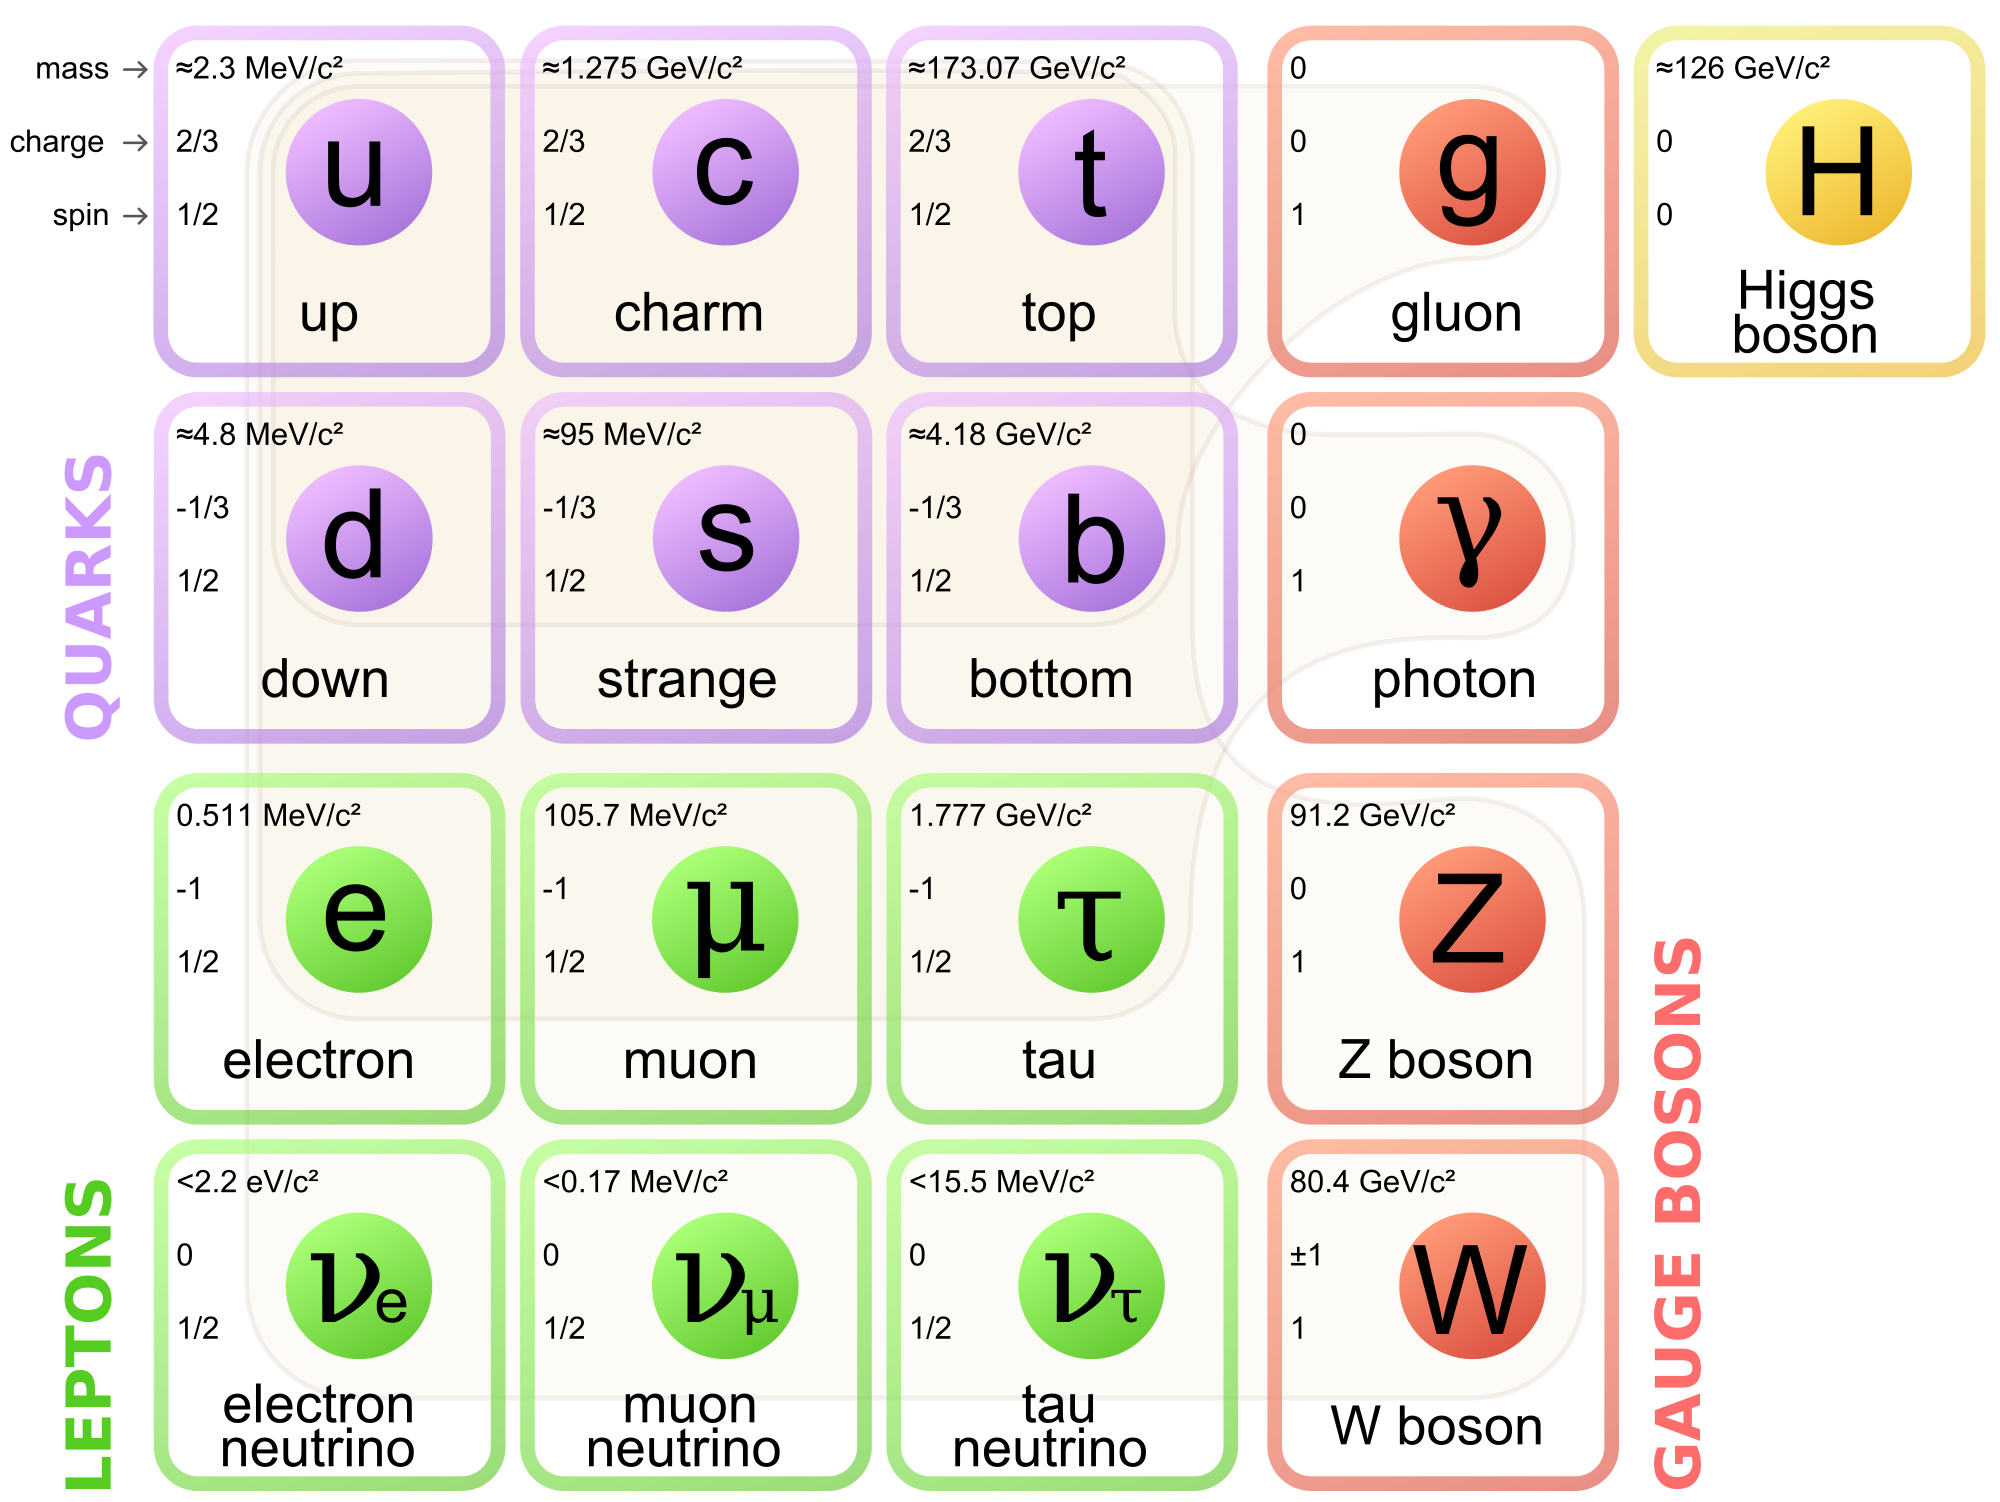
\includegraphics[width=0.9\textwidth]{IntroFigures/TheSM.png}
 \caption{The catalog of particles in the standard model.\label{fig:SMcartoon}}
\end{figure}

The dynamics and kinematics of the SM are controlled by the
Lagrangian density, which in conjunction with the particle content and
force carriers completes the theory. The lagrangian density is
presented below in compact formulation:
\begin{equation}
 \begin{aligned}
        \mathcal{L}_{\mathrm{SM}}& = -\frac{1}{4}B_{\mu\nu}B^{\mu\nu}
        -\frac{1}{4}W^{a}_{\mu\nu}W^{\mu\nu}_{a} - \frac{1}{4}G^{\alpha}_{\mu\nu}G^{\mu\nu}_{\alpha} 
        \qquad \text{gauge terms}\\
        &+\bar{\ell}_{\mathrm{L}}\tilde{\sigma}^{\mu}iD_{\mu}\ell_{\mathrm{L}}
        +\bar{e}_{\mathrm{R}}\sigma^{\mu}iD_{\mu}e_{\mathrm{L}} +
        \bar{\nu}_{\mathrm{R}}\sigma^{\mu}iD_{\mu}\nu_{\mathrm{L}} \qquad \text{lepton kinetic terms}\\
        &+\bar{q}_{\mathrm{L}}\tilde{\sigma}^{\mu}iD_{\mu}q_{\mathrm{L}}
        +\bar{u}_{\mathrm{R}}\sigma^{\mu}iD_{\mu}u_{\mathrm{L}} +
        \bar{d}_{\mathrm{R}}\sigma^{\mu}iD_{\mu}d_{\mathrm{L}} + \qquad \text{quark kinetic terms}\\
        &+\mathcal{L}_{\mathrm{Higgs}} +
        \mathcal{L}_{\mathrm{Yukawa}}\qquad \text{Higgs and Yukawa terms}
       \end{aligned}
\label{eq:theSMlagrangian}
\end{equation}

Where $\ell_{\mathrm{L}}=\begin{pmatrix}e_{\mathrm{L}}\\
  \nu_{\mathrm{L}}\end{pmatrix}$ is the lepton $\mathrm{SU(2)_{L}}$
doublet, $q_{\mathrm{L}}=\begin{pmatrix}u_{\mathrm{L}}\\
  d_{\mathrm{L}}\end{pmatrix}$ is the quark $\mathrm{SU(2)_{L}}$
doublet, $D_{\mu}$ is the corresponding covariant derivative, and
 $\sigma_{mu}$ is the identity and the pauli matrices ($\sigma_{mu} = {1,\sigma^{i}}$).
The $\mathcal{L}_{\mathrm{Higgs}}$ and $\mathcal{L}_{\mathrm{Yukawa}}$
are presented in sections~\ref{higgs} and~\ref{yukawa}, respectively.
Table~\ref{tab:SMGroup} presents the matter field representation in
the SM gauge group.

\begin{table}[htb]
\centering
\large
\begin{tabular}{cccc}
  \hline
  \hline
  field &  $\mathrm{SU(3)_{C}}$ &  $\mathrm{SU(2)_{L}}$ & $\mathrm{U(1)_{Y}}$\\
  \hline                                                        
  $q_{L}$ & $\mathbf{3}$ &  $\mathbf{2}$ & 1/6\\
  $\ell_{L}$ & $\mathbf{1}$ &  $\mathbf{2}$ & -1/2\\
  $u_{R}$ & $\mathbf{\bar{3}}$ &  $\mathbf{1}$ &-2/3\\
  $d_{R}$ & $\mathbf{\bar{3}}$ &  $\mathbf{1}$ &1/3\\
  $e_{R}$ & $\mathbf{1}$ &  $\mathbf{1}$ & 1\\
  $h$ & $\mathbf{1}$ &  $\mathbf{1}$ & 1/2\\
  \hline
  \hline
\end{tabular}
  \caption{\label{tab:SMGroup} Group representation of the matter
    fields in the SM.}
\end{table}
\section{The Higgs Boson and Electroweak Symmetry
  Breaking}\label{higgs}
Gauge theories prohibit -- in order to mantain the local symmetries --  explicit mass terms for the gauge bosons in the SM,
therefore all gauge bosons are massless. Since some of gauge boson in
the SM are massive ($W^{\pm}$,$Z$) there should be a mechanism by
which gauge boson acquire mass. The gauge boson masses in the SM are
realized by the \textit{spontaneous symmetry breaking} of the
$\mathrm{SU(2)_{L}}\times U(1)_{\mathrm{Y}}$ symmetry which induced by the nature of
the Higgs potential~\cite{HIGGES}. The best way to undertand this mechanism (the
Higgs mechanism) is to closely look at the lagrangian density:

\begin{equation}
\label{eq:higgsPotential}
\mathcal{L}_{\mathrm{Higgs}} =
(D^{\mu}\mathbf{\Phi})^{\dagger}(D^{\mu}\mathbf{\Phi}) +
V(\mathrm{\Phi});\hspace{1cm} V(\mathrm{\Phi}) = -\mu^{2}\Phi^{\dagger}\Phi +\lambda(\Phi^{\dagger}\Phi)^{2},
\end{equation}
where $D^{\mu}$ is the covariant derivative; $\Phi$ is a spin-0
complex field, and a $\mathrm{SU(2)_{L}}$ doublet with weak
hypercharge $\mathrm{Y} = 1/2$. The field is more easily represented
as a $\mathrm{SU(2)_{L}}$ doublet in the following fashion:
\begin{equation}
\label{eq:higgdoublet}
\Phi = \begin{pmatrix} \phi^{+}\\
  \phi^{0}\end{pmatrix}.
\end{equation}

When $\mu^{2} > 0$ the potential ($V(\Phi)$) has the commonly known
``Mexican hat'' shape, shown in Figure~\ref{fig:MexHat}, whith a minimum which does not preserve the
original $\mathrm{SU(2)_{L}}\times U(1)_{\mathrm{Y}}$
symmetry. Therefore the scalar field acquires a non-zero
\textit{vacuum expectation value (vev)}:
\begin{equation}
\label{eq:vev}
\langle \Phi \rangle \equiv \langle 0 | \Phi | 0\rangle = \frac{1}{\sqrt{2}}U(x) \begin{pmatrix} 0\\
  v\end{pmatrix}; \hspace{1cm}v = \sqrt{\frac{\mu^{2}}{\lambda}},
\end{equation}

\begin{figure}
 \centering
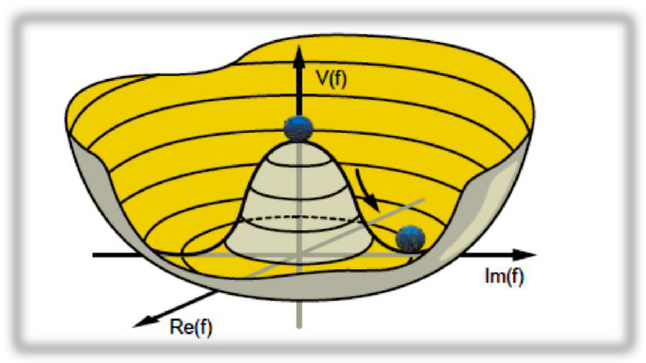
\includegraphics[width=0.9\textwidth]{IntroFigures/MexicanHat.png}
 \caption{The shape of the Higgs potential (``Mexican hat''). The
   degeneracy of the potential is observed along the azimuthal angle\label{fig:MexHat}}
\end{figure}

where $U(x)$ is a unitary transformation that transforms the field
into the degenerate solution. An important consequence is that the
\textit{vev} of field preserves a $U(1)$ symmetry from the original
$\mathrm{SU(2)_{L}}\times U(1)_{\mathrm{Y}}$ symmetry of the
lagrangian. Therefore the full electroweak symmetry of the SM
($\mathrm{SU(2)_{L}}\times U(1)_{\mathrm{Y}}$) is spontaneously broken
to $U(1)_{\mathrm{EM}}$.

This spontaneous breaking of the $\mathrm{SU(2)_{L}}\times
U(1)_{\mathrm{Y}}$ symmetry is responsible for the appearance of
masses to 3 of the four gauge bosons in the electroweak sector, this
is called: the Higgs mechanism. The masses become apparent when
replacing the \textit{vev} into the Higgs kinetic term in the
lagrangian:

\begin{equation}
\label{eq:HiggsMass}
(D^{\mu}\Phi)^{\dagger}(D^{\mu}\Phi) \rightarrow (\partial_{\mu}
-igA_{\mu}^{a}\tau^{a} - ig^{\prime}B_{\mu})^{\dagger}(\partial_{\mu}
-igA_{\mu}^{a}\tau^{a} - ig^{\prime}B_{\mu}) 
\end{equation}
\section{Fermion Masses}\label{yukawa}
\chapter{Supersymetry and Naturalness}
\chapter{Dark Matter and Weakly Interacting Particles}




\section{The Large Hadron Collider}
\section{The Compact Muon Sollenoid}
\subsection{The Tracker System}
\subsection{The Electromagnetic Calorimeter}
\subsection{The Hadronic Calorimeter}
\subsection{The Superconducting Solenoid}
\subsection{The Muon Chambers}
\section{Physics Object Reconstruction}
\section{Dark Matter and Weakly Interacting Particles}
\subsection{Introduction}
\subsection{Cosmological Preliminaries}
\subsection{Observational Evidence for Dark Matter Existance}
\subsection{Supersymmetry}
\subsection{Simplified Models}
\subsection{Effective Field Theories at the LHC}

Write your subsection text here.

\section{Conclusion}
Write your conclusion here.

\end{document}
